\section{Background and Motivation}
\label{sec:motivation}
\subsection{Public Cloud}
\label{sec:public_cloud}
\begin{figure}[tb]
	\centering
	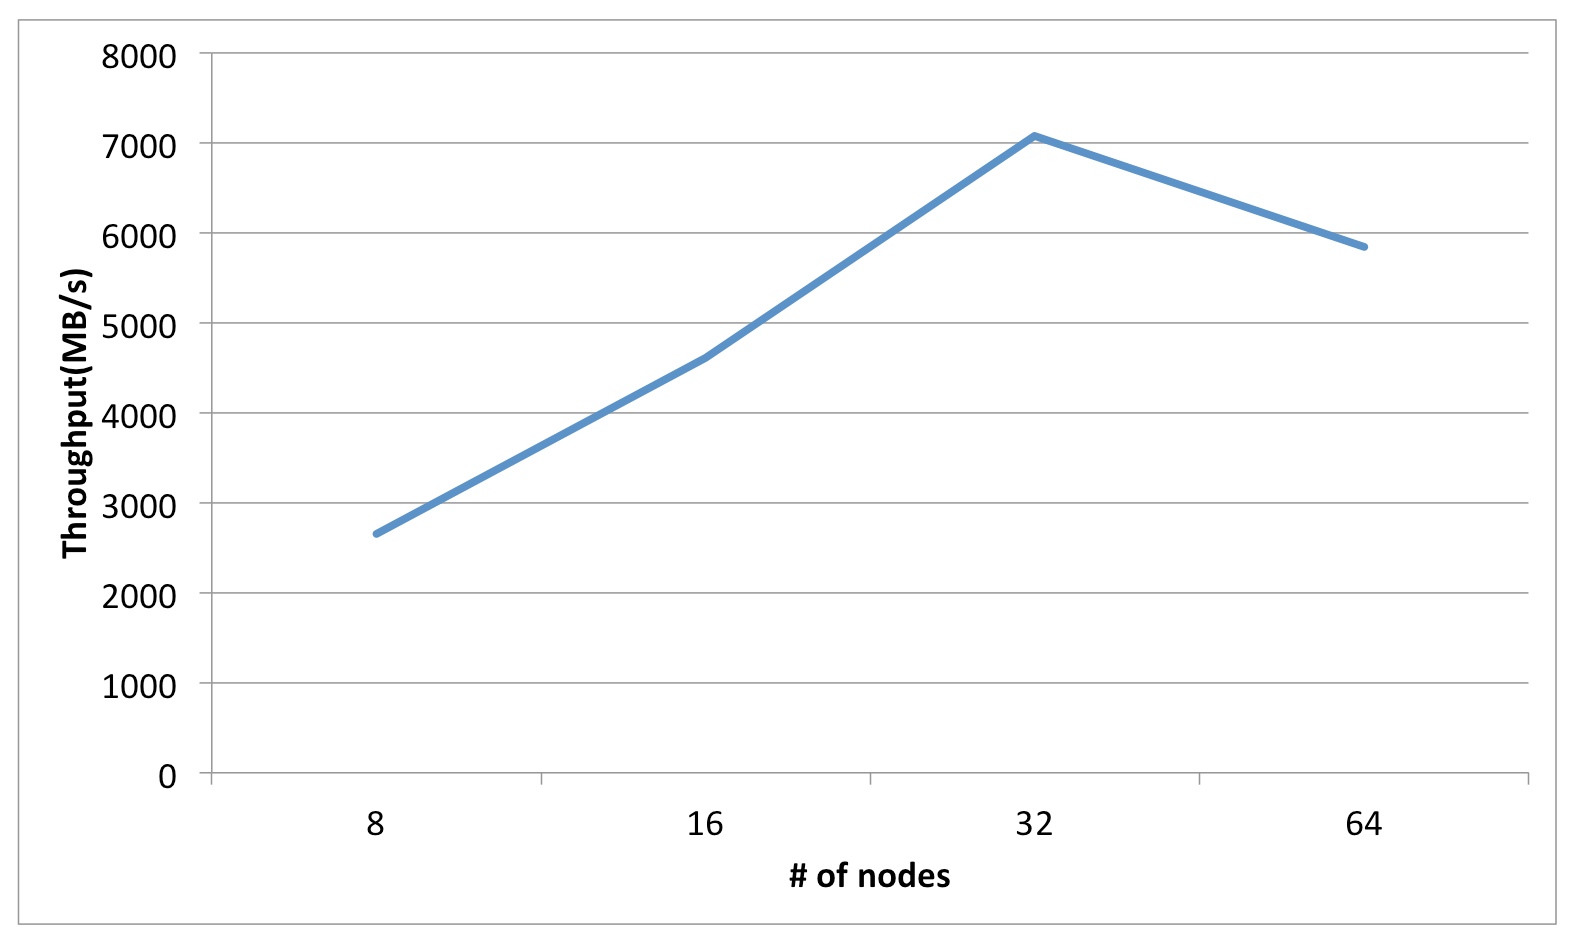
\includegraphics[width=6cm]{../img/throughput_tsubame}
	\caption{I/O Throughput to Lustre inside TSUBAME direct mount}
	\label{throughput TSUBAME}
\end{figure}

\begin{figure}[tb]
	\centering
	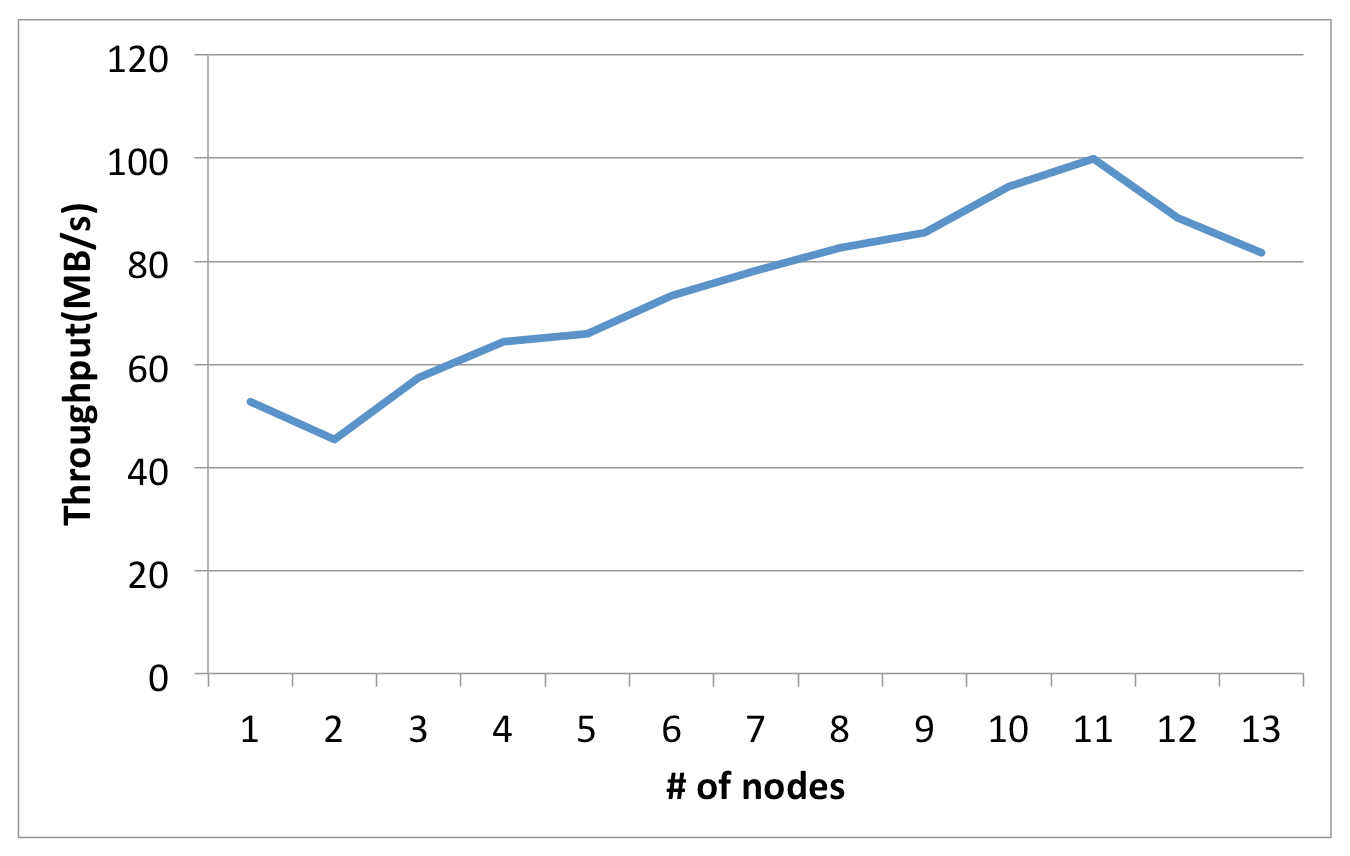
\includegraphics[width=6cm]{../img/AMAZON_to_OUR_LAB}
	\caption{I/O Throughput from AMAZON EC2 to file system inside our lab using sshfs}
	\label{throughput AMAZON to OURLAB}
\end{figure}

\begin{figure}[tb]
	\centering
	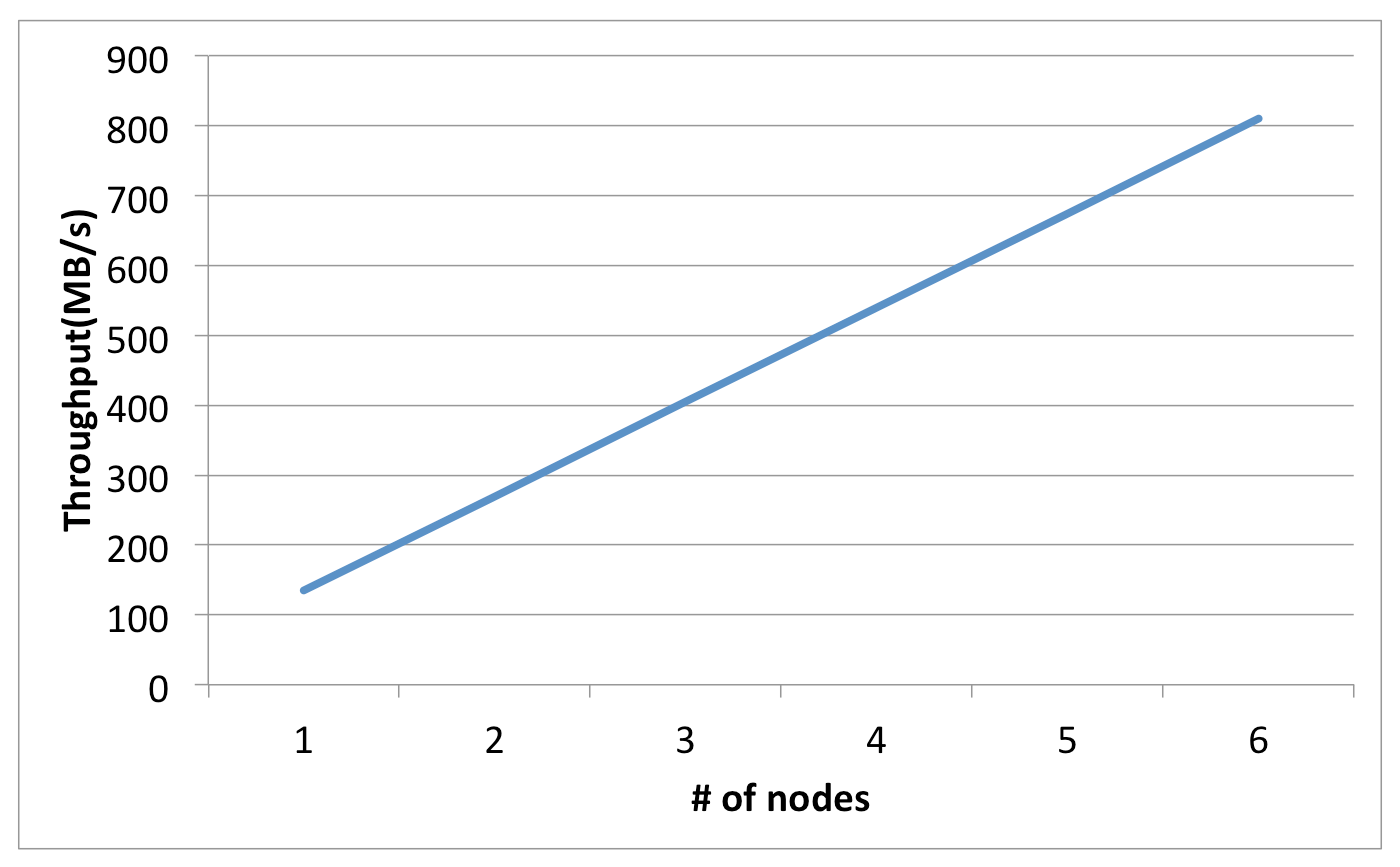
\includegraphics[width=6cm]{../img/point_to_point_AMAZON}
	\caption{point to point connection inside AMAZON}
	\label{point to point connection AMAZON}
\end{figure}

\begin{figure}[tb]
	\centering
	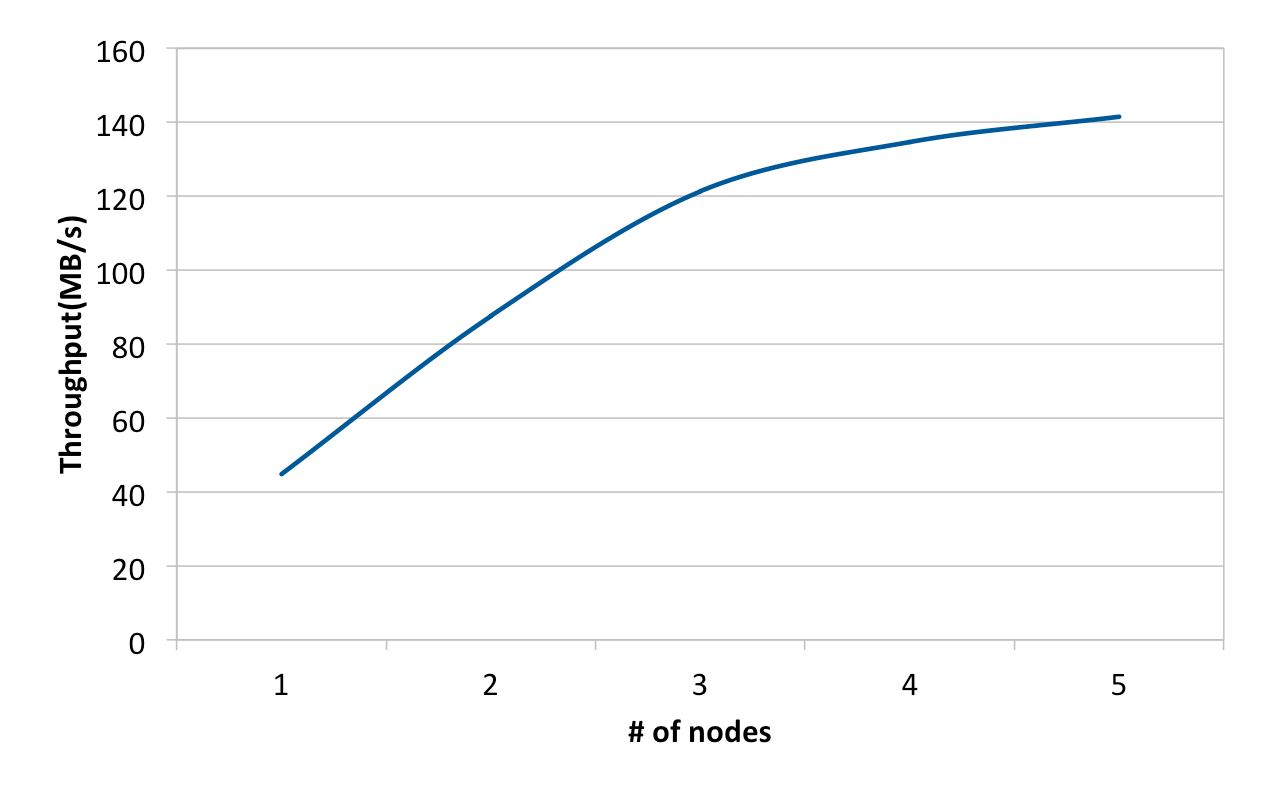
\includegraphics[width=6cm]{../img/point_to_point_lab}
	\caption{point to point connection throughput between AMAZON and our lab}
	\label{point to point connection LAB}
\end{figure}

\begin{table}[h]
\caption{\small TSUBAME thin node specification}
\label{tbl:spec}
\begin{center}
\begin{tabular}{|c|l|}
  \hline
  \cellcolor{lightgray} CPU      & Intel Xeon 2.93GHz CPU (4 cores)*2\\
  %(Hyperthreading enabled)\\
  \hline
  \cellcolor{lightgray} Memory   & 54GB (16 GB)    \\
  \hline
  \cellcolor{lightgray} SSD      & 120GB \\
  \hline
  \cellcolor{lightgray} GPU	 & NVIDIA Tesla K20X *3\\
  \hline
  \cellcolor{lightgray} Network  & QDR InfiniBnd *2 (80Gbps)\\
  \hline
\end{tabular}
\end{center}
\end{table}

\kento{Please explain what Public cloud is with example of Amazon EC2. Then, the details which is needed to mention for readers understand the rest of the sections.
  (1-1) Architecture (VM environment \& datacetners are geographically distributed)
  (1-2) Explain instance types which is related to this paper. Current draft does not mention any instance types.
  (1-3) introduce pay-as-you-go model to help readers understand the cost-based model in the modeling section 
  (1-4) [please add whatever you think it's needed]}
Public cloud is one in which the services and infrastructure such as applications and storage are provided off-site over the Internet, the main benefit of using a public cloud service are: easy fast and inexpensive set-up because hardware, application and bandwidth are covered by the provider, easy to scale to meet needs, no wasted resources because you pay for what you use.
There are many companies provide public cloud solution like google, IBM, Microsoft etc., among them, Amazon Elastic Compute Cloud (Amazon EC2)\cite{AMAZON_AWS} is one of the most famous public cloud, like other public cloud, Amazon EC2 privdes Virtualize computing, and owns computing and data centers in several geographic regions.
Amazon EC2 provide a large amount of instance types optimized to fit different use cases comprise varying combinations of CPU, memory, storage, and networking capacity.
In this study, we used general purpose m3.xlarge instance which has 4 vCPUs, 15GiB memory, 2*80GB SSD storage and high level Ethernet network condition in Tokyo region, we run Amazon Linux AMI 2014.03.2 (HVM), which is based on Linux 3.10 on these instances.
Amazon EC2 charges for nodes usage, Amazon use a pay-as-you-go pricing policy\cite{AMAZON_AWS}, which means you pay only for what you use, there is no minimum fee and you will pay for compute capacity by the hour with no long-term commitments.
\subsection{Federation between supercomputers and clouds}
\kento{Please explain (2-1) how we federate supercomputers with clouds. $=>$ Virtualize supercomputer (e.g. TSUBAME V) + VM on clouds. 
                      (2-2) what the advantages are. $=>$ VMs can provide the same execution environment on both supercomputers and clouds
                      (2-3) [please add whatever you think it's needed]}
When we try to federate supercomputer with public clouds, there are need to have a similiar performance and environment between these two systems.
So we virtualize the supercomputer(like TSUBAME V queue) and federate VMs running on supercomputers with VMs provided by public cloud.
By using VMs, we can run the same image on both supercomputer and public cloud as well as set both the same specification, and make it looks the same to user.%we can use in order to get the same execution environment on both supercomputers and clouds, we virtualize supercomputer, e.g. TSUBAME V queue with VM on clouds.
\subsection{Challenges in Federation with clouds}
\label{sec:problems}
\kento{In this section, (3-1) First explain I/O problems in federation with clouds based on the cloud architecture explained in the above (1-1) as well as using Fig.1-4. 
                        (3-2) Then, please briefly clarfy why ``(A) I/O burst buffer`` can improve I/O performance without using model. For example, parallel I/O, cacheing .... 
                              (Remember we knew that I/O burst buffer is effective before compareing the performances between w/ and w/o burst buffers by using performance model)
                        (3-3) Another challenge is a choice of instance types for burst buffer, and understanding the trade-off between I/O perfomrance and the monetary cost. 
                              In addtion, the choice of instances, the trade-offs are changes depending on given a supercomputer and cloud environments, such as network throughput, PFS performance. 
                              That's why the ``(B) perfomrance modeling`` is important}
Although we virtualize supercomputer and obtain a similiar environment on both supercomputers and clouds, there are still several problems remains, for example, input data of applications running on supercomputer is usually stored in shared storages in the same system and can be read from and wrote to these storages with a extremely high throughput.

We use Iperf\cite{iperf}, which was developed by NLANR/DAST as a modern alternative for measuring TCP and UDP bandwidth performance, and IOR\cite{IOR}, which is widely used for benchmarking parallel file systems using POSIX, MPIIO, or HDF5 interfaces.
Fig.~\ref{throughput TSUBAME} shows read and write throughput from TSUBAME V queue nodes (VM runing on TSUBAME Thin node, which specification is shown in \tabref{tbl:spec}) and TSBUAME Lustre file system, which is mounted by using lustre client, it is a interconnection throughput inside TSUBAME supercomputer, we can see that I/O throughput growing as numbers of nodes growing, and the aggregate read and write throughput reach 6-8GB/s with 64 nodes, the same result also can be seen in \cite{checkpointing}.
However, Fig.~\ref{throughput AMAZON to OURLAB} shows I/O throughput between AMAZON EC2 nodes and a file system machine inside our lab, since TSUBAME Lustre can not be accessed outside of TSUBAME because of security problem, instead of TSUBAME Lustre file system, we used a file server inside our lab, which has 1GBit/s internet bandwidth, also because of security problem, we used sshfs\cite{sshfs},which is a filesystem client based on SSH File Transfer Protocol, to mount this file system from Amazon.
We can see that the I/O throughput also grows as number of nodes grows but the aggregate throughput is only 100-140 MB/s, which is limited by Internet bandwidth, about 40-80 times smaller than throughput inside TSUBAME.
For data-sensitive application, low I/O throughput is devastating, especially for application running on supercomputers, furthermore, lower I/O throughput leads a longer execution time, according to Amazon pay-as-you-go policy, longer execution time means more cost.

However, when we look at Ethernet throughput inside Amazon as Fig.\ref{point to point connection AMAZON} shows, although we only show the result up to 8 pairs of nodes, each node achieved only 135MB/s (1GBit/s), the influence between nodes is extremely small, figure shows a perfect linear line also a strong scalability.
since when we running the benchmark, many other users were also running applications on Amazon, so we can assume that highest throughput 1GB/s (8Gbit/s) shown in Fig.~\ref{point to point connection AMAZON} is not the maximum bandwidth of Ethernet in Amazon EC2 .
Comparing Fig.~\ref{point to point connection AMAZON} with Fig.~\ref{throughput AMAZON to OURLAB} and Fig.~\ref{point to point connection LAB}, Ethernet throughput is much higher than Internet, it shows that our solution, by using I/O buffer nodes can achieve a higher Ethernet throughput than Internet.

To solve this problem, we propose our I/O burst buffer architecture, since usually Internet throuhput is the bottleneck, by using parallel I/O and cacheing file in I/O buffer nodes, we can fully utilize the Internet bandwidth as well as avoid frequently transfering file between two systems, hence achieve a high I/O throughput.
Althought using I/O buffer can increase I/O throughput, reduce the execution time and cost, I/O buffer nodes will be charged for usage, also a better instance will cost more than a normal one, there will be a trade-off between I/O performance and monetary cost, we will introduce a throughput-based model and a cost-based model to predict the throughput and overall cost.
%Moreover, the instance choice, number of I/O nodes depends on supercomputer and pulic cloud environment, in our following section, we will provide a performance modele

%when we try to move some jobs to public clouds after federation, the data 
\kento{Then, in the rest of the section, we explain (A) and (B)}


%\subsection{(Current Section 2)}
\kento{Please fit the below sentences to the above sections with additional explanations}

% vector figures
% Fig. 4 does not have a frame
% write machine spec 

%When people analyze large size of data, parallel programme is widely used in order to reduce computation time, especially when using supercomputer.
%However, it is usually difficult for a non-computer-scientist to write a parallel program, or re-write some existing applications into parallel version.
%Many serial applications are submitted to Supercomputer and occupy computing nodes for a long time, causing other applications which offer large number of nodes to wait for nodes, and leading a low utilization of computing resource.
%Consider following situation, there are 50 nodes available when a user submits a serial program using 1 node for 4 hours, after an hour a user try to run a program using 50 nodes, then he can't start his program until the first user finished his job.
%Such situation happens frequently when thousands and hundreds of users using one system at the same time and leading a low utilization of computing resource.
%One solution is running several virtual machines on a single physical machine for increasing utilization, which is used in TSUBAME Supercomputer, but sometime it still can't meet the request.
%For request not always reaches peak, it is not wise to increase nodes just for a temporary request peak.
%However even using virtual machines computing nodes still can't meet the request of users, for example, power problem will be critical in summer and nearly half of computing nodes have be shut down to reduce electricity consumption in the case of TSUBAME Supercomputer.
%Facing these problems, one solution will be federate supercomputer with public cloud.
%By using public cloud computing nodes just in request peak or when facing with power problem, people can save cost for buying new machines.
%Of cause, there will be many challenges when Supercomputer federates with public cloud, such as security problems, using public cloud may cause research data opened to public, also connecting with Internet put Supercomputer under threats of hacker's attack.

%Data shown in this section is taken from AMAZON EC2 m3.medium nodes, which have 3.75GiB memory and Moderate Network Performance and TSUBAME 2.5 V queue, which uses VM.


%Fig.~\ref{throughput TSUBAME} shows I/O throughput between TSUBAME V queue nodes \kento{Describe node specification in Table I}(VM runing on TSUBAME Thin node, which specification is shown in \tabref{tbl:spec}), which run on VM on several shared machines and TSBUAME Lustre file system, which is mounted by using lustre client, it is a interconnection throughput inside TSUBAME supercomputer, we can see that I/O throughput growing as numbers of nodes growing, and the aggregate read and write throughput reach 6-8GB/s with 64 nodes, the same result also can be seen in \cite{checkpointing}.
%On the other hand, Fig.~\ref{throughput AMAZON to OURLAB} shows I/O throughput between AMAZON EC2 nodes and a file system machine inside our lab, which has about 1GBit/s Internet access.
%From Fig.~\ref{throughput TSUBAME} and Fig.~\ref{throughput AMAZON to TSUBAME Lustre} we can see that the I/O throughput of interconnection inside supercomputer is quit larger than that from AMAZON.
%Also, if we compare the one nodes I/O throughput, 
%Also if we compare Fig.~\ref{point to point connection LAB} with Fig.~\ref{throughput AMAZON to OURLAB}, the maximum throughput \kento{??}
%If we move some jobs to AMAZON EC2 with input data stored in TSUBAME Lustre, the execution time will increase because of I/O low throughput,for a data sensitive application, it will be devastating, also according to AMAZON's pay-as-you-go policy\cite{AMAZON_AWS}, longer execution time means more cost.

%But when we compare Fig.~\ref{point to point connection TSUBAME} with FIg.~\ref{point to point connection AMAZON}, the interconnection throughput 

%using I/O burst buffer requires addtional nodes running on public cloud and means more cost, also like Amazon EC2, public cloud usually provides various instance types with different specification, using which instance type also will affect both cost and performance.
%We provide a cost-based model to determine 
%Since we can achieve a high interconnection throughput inside a system (HPC system, public cloud), we consider use some nodes as a buffer nodes, using a buffer queue to buffer I/O data and achieve a high throughput.

%Although there are some studies about workflow optimization and  balance\cite{Workload}, Since data transfer rate is extremely low in Internet compared with interconnection network and data size processed is extremely large, user do not want to settle their nodes across two systems, so in this model, we just consider the situation that all nodes used for the same job are allocated in the same system.
